\documentclass[addpoints,12pt]{exam}
\pagestyle{empty}
\usepackage{amsmath}
\usepackage{amssymb}
\usepackage{latexsym}
\usepackage[dvips]{graphicx}
\usepackage{enumerate}
\usepackage{amsfonts}
\newcommand{\nl} {\newline}
\newcommand{\normal}{\triangleleft}
\newcommand{\homo}{\simeq}
\newcommand{\R}{\mathbb{R}}
\newcommand{\Z}{\mathbb{Z}}
\newcommand{\Q}{\mathbb{Q}}
\newcommand{\N}{\mathbb{N}}
\newcommand{\C}{\mathbb{C}}
\newcommand{\ov}{\overline}
\newcommand{\E}{\varepsilon}
\newcommand{\F}{\varphi}
\newcommand{\MF}{\mathbb{F}}
\newcommand{\s}{\sqrt}

\everymath{\displaystyle}
\input{../../../AxesFunction}

\def\arraystretch{2}
\setlength\arraycolsep{20pt}
%\renewcommand{\baselinestretch}{1.3}

\begin{document}

~\hfill Student Name: \rule{2in}{.1pt}\\\\
\phantom{.}\hfill PERM: \rule{2in}{.1pt}\\\\
%\phantom{.}\hfill Section Time (e.g. 8am): \rule{2in}{.1pt}\\
Circle the section you ATTEND (if you are enrolled a different section, note which one):
\vskip.15in

\textbf{\begin{tabular}{cccccc}
Kyle: & Tue:8am & Tue:4pm & Tue:7pm\\
David: & Tue:5pm & Tue:6pm\\
Yihan: & Mon:4pm & Mon:5pm & Mon:6pm & Mon:7pm\\
Tom: & Tue:8am & Tue:4pm & Wed:8am\\
Matt: & Tue:5pm & Tue:6pm & Tue:7pm\\
\end{tabular}}
\vskip.25in



%Spring 2011
%Instructor: Stepan Paul
%Circle Your Section:\quad 8AM:Rahul\quad 4PM:Rahul\quad 5PM:Rahul\quad 6PM:Rahul\quad 6PM:Brandon
%\vskip0.5truein

\centerline{\bf \underline {Math 4B, Midterm 1, Spring 2017}}

\centerline{\bf \underline{Version B}}
\vskip0.2in

\underline {Instructions}: Read the instructions for each question carefully. No calculators, cell phones, or other electronic devices are permitted. No notes or textbooks. Academic dishonesty will not be tolerated. Show your work, write legibly, and circle your answers. 

\vspace{.5in}
\centerline{\gradetable}

\vspace{.5in}

\textbf{I understand UCSB's policies regarding academic dishonesty, and I certify that this test was taken with academic integrity.}
\vspace{.5in}

Sign and date: \rule{5in}{.5pt}

%\medskip
%\medskip \vskip0.25truein
%\vskip0.25truein

%\vspace{0.5in} \large{\centerline{\begin{tabular}{|c|c|c|} \hline
%Problem  & Points & Score
%\\ \hline
% 1 & 25 &     \\ \hline
% 2 & 10 &      \\ \hline
% 3 & 15 &      \\ \hline
% 4 & 10 &      \\ \hline
% Total & 60 &  \\ \hline
%\end{tabular}}}
%}

\newpage
\begin{questions}

\question[10] Find the general solution to the ODE:

$$y'=y^2\cos t$$
\newpage

\question[10] Solve the initial value problem

$$y'=xe^{-\cos x}+y\sin x,\quad y(0)=3$$

\newpage

\question[6] In this problem, you need to set up a differential equation modeling the biomass $M$ of trees in Tillamook State Forest in Oregon as a function of time $t$ based on the following information.
 \begin{itemize}
  \item Natural tree growth causes biomass to increase at a constant rate.
  \item Logging permits are issued in such a way that allows biomass to be removed a rate proportional to the total biomass.
 \end{itemize}
 
 \begin{parts}
  \part Write down your differential equation and \textbf{one} complete sentence explaining it.
  \vfill
  
  \part Sketch the phase line for your differential equation.
  \vfill
  
  \part According to this model, what long-term prediction can you make about the biomass in the forest? Answer with \textbf{one} complete sentence.
  \vfill
  
 \end{parts}
 
 \newpage

\question[8] Answer the following questions about the ODE
$$y'=\sqrt y - 2e^{t}$$

\begin{parts}

 \part Below is an incomplete table in which Euler's method is being used. Fill in the three blanks.
 
 $\begin{array}{|c|c|c|}
  \hline
  t & y & y' \\
  \hline
  0 & 36 & \\
  \hline
  0.5 & & 2.86\\
  \hline
  1 & & 0.84 \\
  \hline
  1.5 & 39.86 & -0.66\\
  \hline
 \end{array}$
 
 \vfill
 
 \part Suppose $y=f(t)$ is a solution to this differential equation, and that $f(t)$ has a local maximum at $t=5$. What is the value of $f(t)$ at this maximum?
 \vfill\vfill\newpage

 \part Circle the slope field that matches this ODE:\\
 \setlength\tabcolsep{20pt}
 
\begin{tabular}{c|c} 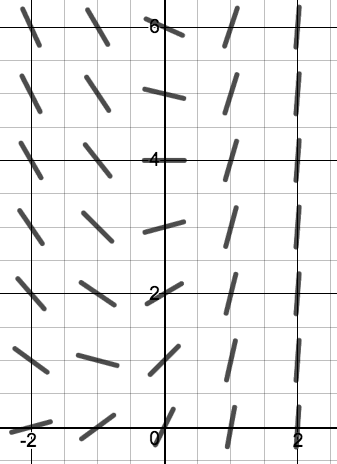
\includegraphics[height=3in]{sf2} & 
 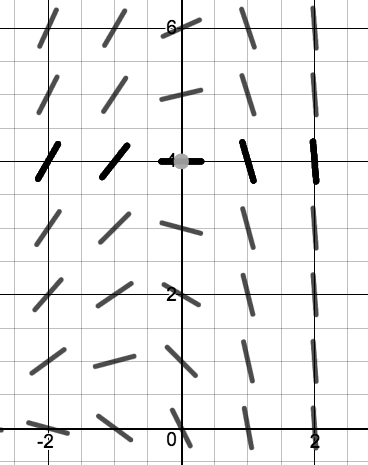
\includegraphics[height=3in]{sf1}\\
 A & B \\
 \hline
 ~\\
 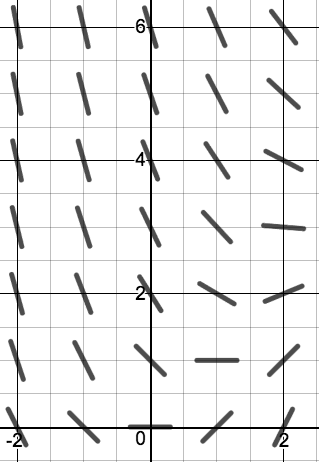
\includegraphics[height=3in]{sf4}&
 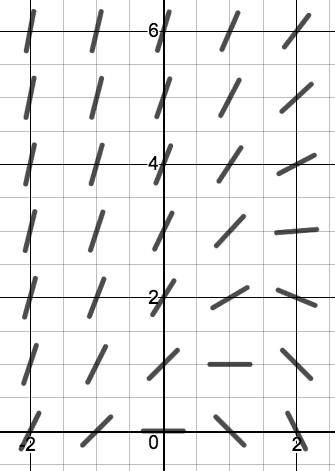
\includegraphics[height=3in]{sf3}\\
 C & D
 \end{tabular}
 
 
\end{parts}

\newpage


 
 \question[5] DO ONE AND ONLY ONE of the following two problems. If you do both, we will just grade the first one. CLEARLY INDICATE which problem you are doing by CIRCLING that problem.
 \begin{parts}
  \part Find the general solution to the following ODE by making the substitution $v=\frac{y}{x}$.
  $$y'=\frac{xy-3y^2}{x^2}$$
  \vfill
  \part Find the general solution to the following ODE. You should solve for $y(x)$ explicitly. Hint: think about exactness.
  $$(2xy-\cos x)+(x^2+1)y'=0$$
  \vfill
 \end{parts}

\end{questions}

\newpage

If you finish early, you must stay in your seat until the end. You should check your work, but if you are done, you can amuse yourself by coloring in these regular pentagonal tilings.

\begin{tabular}{cc}
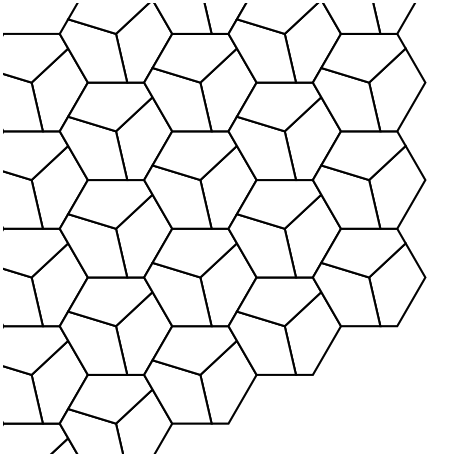
\includegraphics[width=.4\textwidth]{T1} & 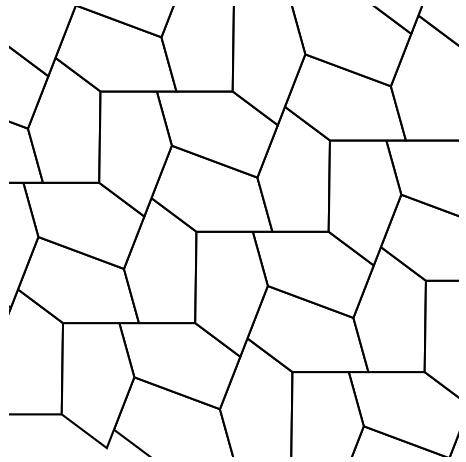
\includegraphics[width=.4\textwidth]{T2} \\
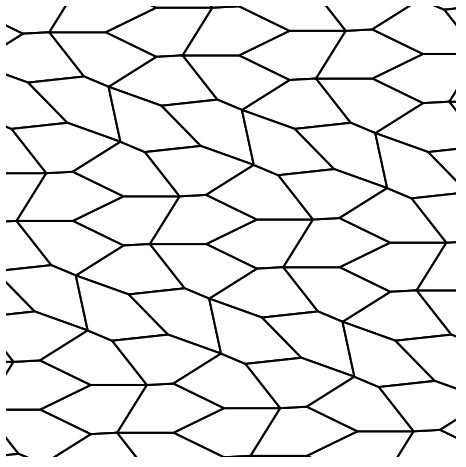
\includegraphics[width=.4\textwidth]{T3} &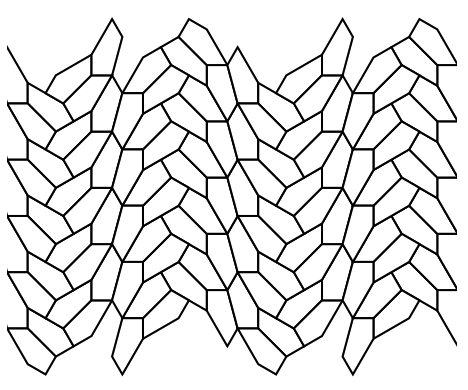
\includegraphics[width=.4\textwidth]{T15} 
\end{tabular}
\end{document}
